\chapter{Back-End}
Für die Entwicklung des Backends standen C++ und Python im Raum. Auf Empfehlung unseres Betreuers hin und aufgrund der einfachen Implementierung einiger Beispiele entschieden wir uns für die Entwicklung in Python.
\section{Konzept}
\section{Verwendete Open-Source Bibliotheken}
\subsection{OpenCV}
Bei OpenCV (Open Source Computer Vision Library) handelt es sich um eine Bibliothek zur Verarbeitung und Bearbeitung von Bildern und Video-Formaten. OpenCV wurde in C/C++ entwickelt und unterliegt derzeit einer Lizenz, die eine kostenlose Nutzung für akademische als auch kommerzielle Zwecke ermöglicht. Die Bibliothek unterstützt nicht nur herkömmliche Betriebssysteme wie Windows, Linux und Max OS, sondern auch Mobile Betriebssysteme wie iOS und Android. OpenCV wurde so entwickelt, dass es effizient in Echtzeitsystemen genutzt werden kann. In unserem Projekt werden wir für die Bearbeitung des Video-Streams mehrere Funktionalitäten der Bibliothek aufgreifen und verwenden.
\subsection{Numpy}
Bei NumPy handelt es sich um eine Python-exklusive Bibliothek. Diese wurde entwickelt, um mathematische Funktionen anzuwenden. Der Schwerpunkt hierbei liegt ins besonders auf Matrizen. Auch Numpy unterliegt der gleichen Lizenz wie OpenCV und erlaubt daher eine kostenlose Nutzung. In unserem System benötigen wir Numpy um ein paar Operationen auf unsere Bilder anzuwenden, oder auch um exemplarisch Bilder zu erstellen.
\section{Bildverarbeitungsprozess}
Um eine Bewegung aus mehreren Bildern erkennen zu können, reicht es normalerweise aus, die jeweiligen Pixelpositionen voneinander zu subtrahieren. Hat man an diesem Punkt noch weiße bzw. farbige Pixel, kann man davon ausgehen, dass es einen Unterschied gibt und daher auch eine Bewegung vorhanden ist. Da wir nun die Bewegungserkennungen einer Kamera umsetzen sollen, kann man nicht so simpel vorgehen. Es gibt mehrere kleinere Aspekte die beachtet werden können und es gibt auch keine einfache Lösung für einige Probleme. Im Laufe dieses Kapitels werden einige Probleme beleuchtet sowie Lösungen für diese aufgeführt, sofern umsetzbar.

\begin{figure}[ht]
	\flushright
	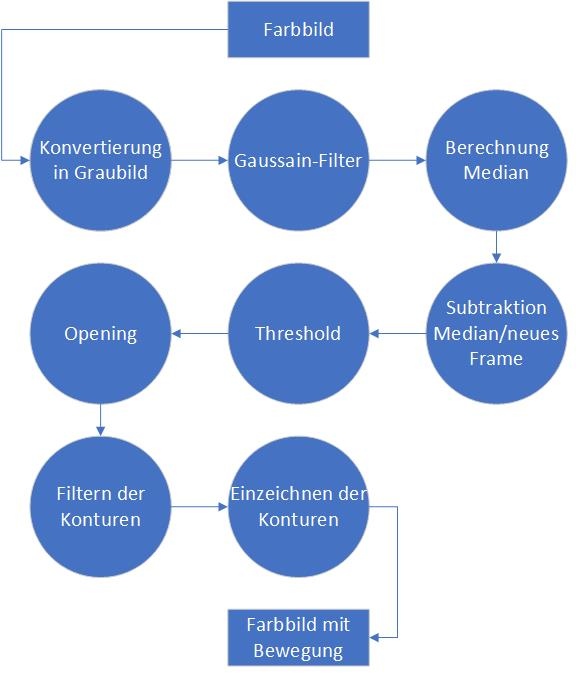
\includegraphics[]{content/pictures/Bildverarbeitung.jpg}
	\caption{Ablaufdiagramm der Bildverarbeitung}
\end{figure}

In dem Ablaufdiagramm kann man die Vorgehensweise unserer Bildverarbeitung sehen. Der erste Schritt beinhaltet die Konvertierung eines Farbwertbildes in ein Grauwertbild. Diese kann mit Hilfe von OpenCV leicht umgesetzt werden. Somit muss man sich keine Gedanken um den Datentyp des Bildes machen. Der Sinn hinter dieser Konvertierung bezieht sich stark auf die Performanz der kommenden Operationen, welche für die Bewegungserkennung notwendig sind. Würden wir alle Operationen mit einem Farbwertbild durchführen, hätten wir mindestens eine dreimal längere Laufzeit für die Bildverarbeitung.
Als nächsten Schritt entfernen wir das Rauschen aus dem Grauwertbild. Bei Rauschen in einem Bild handelt es sich um Pixelfehler die Werte enthalten, die dem eigentlichen Farbschema widersprechen. Diese entstehen meist direkt durch das Aufnahmegerät. Mithilfe des in OpenCV gebotenen Gaussain-Filters können diese bereinigt werden. Hierbei werden die umliegenden Pixel angeschaut und anhand denen entschieden, welchen Wert er erhalten wird. Sprich liegt der Pixel in einer dunklen grauen Fläche wird auch der Pixelwert den entsprechenden Grauwert erhalten.
Da wir nun das neue Bild vorbereitet haben, benötigen wir noch das vorherige Bild für den Vergleich. In unserem Fall berechnen wir Pixelweise den Median aus den letzten 15 Bildern. Durch dieses Vorgehen sollen kleinere Bewegungen von der Bewegungserkennung ignoriert werden. Für das Speichern der Bilder nutzen wir eine zyklische Liste, die das älteste Objekt beim überschreiten der maximalen Anzahl entfernt. Für die Berechnung des Medians bietet OpenCV leider keine Funktion. Daher greifen wir auf die Bibliothek NumPy zurück. Diese ermöglicht uns sowohl die Addition als auch das Berechnen des Medians. Gibt es keinen Fehler bei der Berechnung wird uns das berechnete Bild zurückgegeben, ansonsten erhalten wir das zuletzt hinzugefügte Bild zurück.
Haben wir nun das Median-Bild und das letzte Bild, können wir diese voneinander subtrahieren. Somit haben wir die Unterschiede aus den letzten Bildern. Die Subtraktion können wir direkt mit OpenCV ausführen.
Als Ergebnis der Subtraktion erhalten wir ein Bild mit unterschiedlichen Grauwerten. Wenn Grauwerte voneinander abgezogen werden, kann es sein, dass ähnliche Grauwerte trotzdem einen Grauwert größer als „0“ zurückgeben. Für uns spielen aber größere Änderungen eine Rolle. Um die niedrigen Grauwerte zu filtern, kann ein Threshold angewandt werden. Durch die Threshold-Funktion von OpenCV ist es uns möglich die Grauwerte mit einer Grenze in Schwarz und Weiß aufzuteilen.  Sprich alle Grauwerte  bis Beispielsweise dem Wert von 30 werden zu schwarz und alle höheren Grauwerte werden weiß.
Da wir kleine Bewegungen nicht als Bewegung zählen lassen wollen, müssen wir kleine Bereiche vorher entfernen. Durch die sogenannte Opening-Operation können kleine Bereiche gefiltert werden. Hierbei werden zuerst alle Bereiche erodiert und die übriggebliebenen Bereiche werden dilatiert. Dadurch bleiben die größeren Bereiche bestehen und kleine Bereiche werden entfernt. OpenCV bietet für die Erosion und Dilatation separate Funktionen an, die sich leicht verwenden lassen.
Als letzten Schritt Extrahieren wir, falls vorhanden, übrig gebliebene Konturen. Gibt es eine Kontur, gab es auch eine Bewegung, und die Pixelkoordinaten der Konturen werden in das Farbwertbild übernommen, um die Bewegung kenntlich zu machen und gegebenen falls werden Empfänger per E-Mail benachrichtigt.
\section{Performanceprobleme durch GIL}
Bei der Berechnung des Medians könnten sinnvoll mehrere Kerne benutzt werden. Dies müsste in Python jedoch über Umwege von Hand gemacht werden, da Multithreading durch den Global Interpreter Lock auf einen Kern beschränkt ist. Bei einem Versuch, bei dem für die Berechnung die Bilder in vier Teile aufgeteilt und eigene Prozesse erstellt wurden, erhöhte sich die Berechnungszeit sogar. Aufgrund des engen Zeitplans konnte dem Versuch der Performanceverbesserung nicht weiter nachgegangen werden.
\section{Zusätzliche Features}
\subsection{Video, Log und Thumbnail}
Es gibt mehrere Aspekte die wichtig für die Bildverarbeitung sind. Da wir über das Backend die Bilder für das Frontend zu Verfügung stellen und auch das Video erstellen, muss einiges in dieser Hinsicht beachtet werden. Zu Beginn haben wir sofort Video, Log und Thumbnail bei der ersten Bewegungserkennung zu Verfügung gestellt. Dies hatte zur Folge, dass beim Aktivieren des Videos die Aufnahme nicht fertiggestellt wird. Und kein Video angezeigt wird. Um dies zu umgehen, werden Video, Log und Thumbnail nur beim Abschluss der Bewegungssequenz weitergeleitet und das Thumbnail kann ein Bild mitten in der Bewegung darstellen.
\subsection{FPS-Berechnung}
OpenCV bietet eine Schnittstelle zum Erstellen von Videos. Hierbei muss vorab eine feste FPS (Frames Per Second) angegeben werden. Während den Tests ist uns aufgefallen, dass das Backend je nach System unterschiedlich schnell arbeitet. Zusätzlich dazu ist die Geschwindigkeit des Videos durch eine falsche Bearbeitungsrate verzerrt. Um dies zu vermeiden, berechnen wir die durchschnittliche FPS zur Laufzeit. Die ersten hundert benötigten Zeiten werden in einer Liste abgespeichert und am Schluss dividiert. Anhand dieses Wertes erhalten wir einen guten Wert, der auch das Video in einer angemessenen Geschwindigkeit darstellt.
\subsection{Maximale Cliplänge}
Um eine maximale Cliplänge gewährleisten zu können muss die Bearbeitungsrate aufgegriffen werden. Wurden genug Bilder gesammelt (FPS x maximale Cliplänge in Sekunden) wird das Video abgebrochen und eine neue Aufnahme wird gegebenenfalls gestartet.
\subsection{Wait for Motion-end}
Wurde gerade eine Bewegung erkannt und die Bewegungen haben aufgehört, wartet die Bearbeitung noch einen Moment ab, ob nicht doch noch eine Bewegung auftaucht. Dadurch wird die Aufnahme nicht direkt beendet, wenn keine Bewegung mehr erkannt wird und ein eventuell kurzer Aussetzer der Bewegung wird ignoriert.
\section{Datenhaltung und Speicherung}
Für die Datenhaltung wurde ein Singleton-Objekt mit den verschiedenen zu teilenden Daten erstellt. Um die Integrität der Daten zu gewährleisten musste darauf geachtet werden, dass keine Zugriffe gleichzeitig auf die jeweiligen Daten
gemacht werden können. Hierfür wurden Locks für die jeweiligen Datenobjekte erstellt.\\
Bei der Erstellung eines Backups dürfen ebenfalls keine Änderungen vorgenommen werden, weshalb alle Locks gesperrt werden müssen.\\
Die Daten müssen für die Anfrage passend zurückgegeben werden.
Damit die Daten nach dem Beenden des Programms noch vorhanden sind, sollten diese gespeichert werden. Da die Daten für die Kommunikation in JSON serialisiert werden müssen, wird auch für das Speichern ein JSONEncoder verwendet. Da die zu speichernden Attribute
der Objekte bereits serialisierbar sind, musste kein eigener Encoder geschrieben werden. Für die Decodierung musste jedoch eine Funktion geschrieben werden, welche die Art der Objekte anhand eines Keys prüft und aus den JSON-Daten wieder Objekte erstellt.
Es gibt drei JSON-Dateien mit denen die Emails, Logs sowie Einstellungen gespeichert werden.
\section{Mailclient}
Ein wesentlicher Teil eines Überwachungssystems ist die Benachrichtigung wie z.B. per Email.
Hierfür haben wir mit Hilfe der umfrangreichen Standardbibliothek in Python einen SMTP-Client erstellt.
Der Mailclient soll zum einen den Benutzer benachrichtigen, wenn eine Bewegung erkannt wurde und zum anderen wenn der maximal zu nutzende Speicher belegt ist.
Beim Start des Backends werden Login und Passwort abgefragt. Für Testzwecke wurde der Anbieter auf unseren verwendeten Provider vorbelegt.
\section{Webserver}
Für die Kommunikation mit dem Frontend sollte eine REST-Schnittstelle definiert werden. Hierzu wurde zuerst mit einem in den Standardbibliotheken verfügbaren HttpServer experimentiert,
welcher jedoch zu minimalisisch und dadurch für die Anwendung ungeeignet war. Anschließend wurde ein Flask-Webserver verwendet, bei welchem recht einfach über das Web Server Gateway Interface die Ressourcen definiert,
und auf diese Ressourcen bestimmte Funktionen registriert werden können. Am einfachsten ginge das mit Annotationen, wenn der Webserver als eigenes Programm läuft. Dies war in unserem Szenario jedoch nicht gegeben, weshalb der Webserver als Klasse definiert und die Pfade innerhalb des Konstruktors hinzugefügt wurden.\\
Der Webserver holt sich durch Anfragen die Daten vom Singleton-Objekt und sendet regelmäßig das aktuelle JPEG für den Videostream.
Allerdings gilt zu beachten, dass der von uns verwendete Webserver nicht für Produktivsysteme gedacht ist.

\section{Videoquelle}
\subsection{Voraussetzung}
Als Videoquelle bieten die meisten IP-Kameras die Bilder als MJPEG oder RTSP-Stream an.\\
Beide Formate werden durch OpenCV und somit durch unsere Anwendung unterstützt.
Ebenso kann OpenCV auch Videodateien unterschiedlicher Formate wie z.B. mp4 oder webm abspielen.
Von einer Youtube-Url kann jedoch nicht gestreamt werden, da Youtube nicht das File direkt zur Verfügung stellt.\\
Der Stream sollte mindestens 15 FPS zur Verfügung stellen, da wir somit auch den Median über den Zeitraum von etwa. einer Sekunde bilden. Wenn der Stream weniger Bilder sendet, wird der Median über einen längeren Zeitraum gebildet und somit ändert sich das Verhalten der Bilderkennung.

\subsection{Auflösung}
Aufgrund der o.g. Performanceprobleme ist die Verwendung einer höheren Auflösung ein großes Problem.\\ Für die Verwendung einer einfachen Bewegungserkennung reicht die Auflösung von 640x368 aus, jedoch erreichen wir selbst hierbei je nach Rechner nur ca. 20 FPS.